\documentclass[tikz,border=10pt]{standalone}
\usepackage{mathpazo}
\usepackage{tikz}
\usetikzlibrary{shapes,arrows,positioning,calc,fit,backgrounds}

\begin{document}

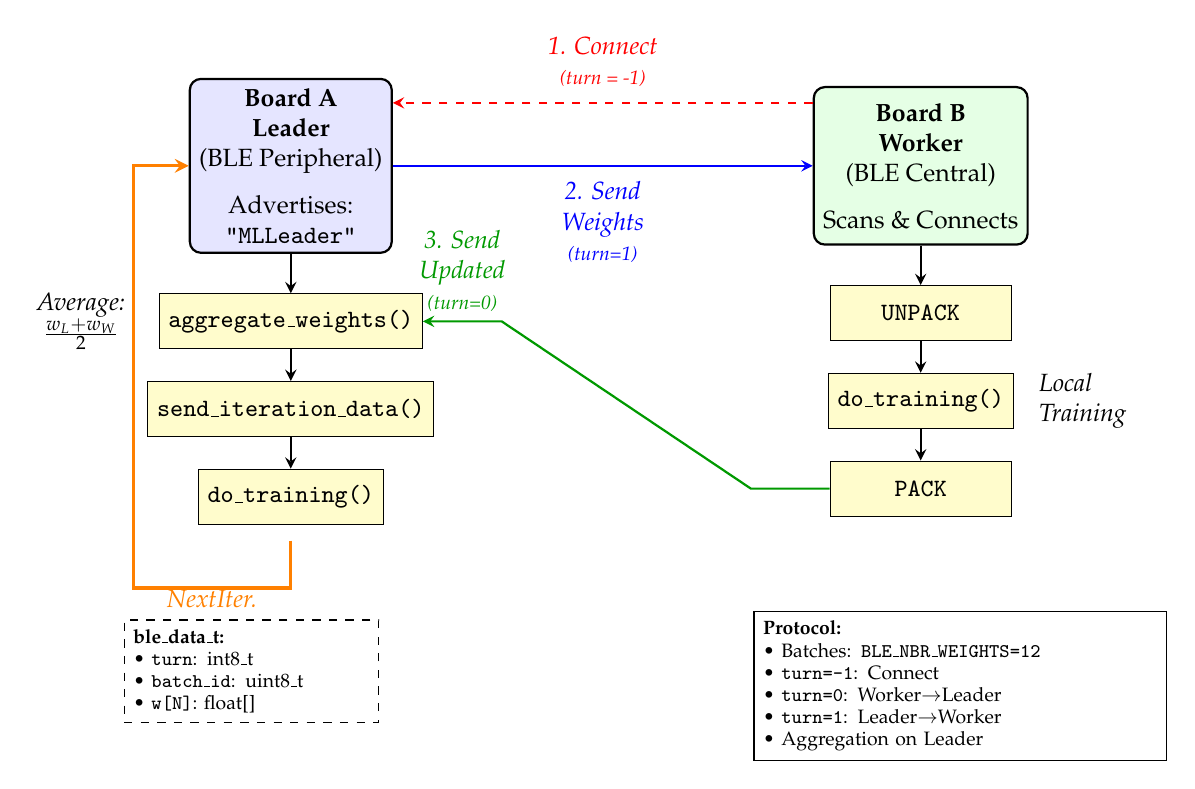
\begin{tikzpicture}[
    node distance=0.6cm,
    box/.style={rectangle, draw, thick, minimum width=2.5cm, minimum height=2cm, align=center, rounded corners, font=\small},
    leader/.style={box, fill=blue!10},
    worker/.style={box, fill=green!10},
    process/.style={rectangle, draw, fill=yellow!20, minimum width=2.3cm, minimum height=0.7cm, align=center, font=\small},
    arrow/.style={->, >=stealth, thick},
    dashedarrow/.style={->, >=stealth, thick, dashed},
    label/.style={font=\small\itshape}
]

% Board A (Leader)
\node[leader] (boardA) at (0,0) {
    \textbf{Board A}\\
    \textbf{Leader}\\
    (BLE Peripheral)\\[0.2cm]
    \small Advertises:\\
    \texttt{"MLLeader"}
};

% Board B (Worker)
\node[worker] (boardB) at (8,0) {
    \textbf{Board B}\\
    \textbf{Worker}\\
    (BLE Central)\\[0.2cm]
    \small Scans \& Connects
};

% Board A process boxes (vertical chain)
\node[process, below=0.5cm of boardA] (aggA) {\texttt{aggregate\_weights()}};
\node[process, below=0.4cm of aggA] (sendA) {\texttt{send\_iteration\_data()}};
\node[process, below=0.4cm of sendA] (trainA) {\texttt{do\_training()}};

% Board B process boxes (vertical chain)
\node[process, below=0.5cm of boardB] (unpackB) {\texttt{UNPACK}};
\node[process, below=0.4cm of unpackB] (trainB) {\texttt{do\_training()}};
\node[process, below=0.4cm of trainB] (packB) {\texttt{PACK}};

% Communication arrows
% Step 1: Connect (turn=-1) - positioned higher
\draw[dashedarrow, red] ($(boardB.west)+(0,0.8)$) -- node[above, label, align=center, yshift=2pt] {1. Connect\\{\scriptsize (turn = -1)}} ($(boardA.east)+(0,0.8)$);

% Step 2: Send Weights (turn=1) - positioned lower, separated from red line
\draw[arrow, blue] ($(boardA.east)+(0,0)$) -- node[below, label, align=center, yshift=-2pt] {2. Send\\Weights\\{\scriptsize (turn=1)}} ($(boardB.west)+(0,0)$);

% Step 3: Send Updated (turn=0) - horizontal line between packB and aggA
\draw[arrow, green!60!black] (packB.west) -- ($(packB.west)+(-1,0)$) -- ($(aggA.east)+(1,0)$) -- (aggA.east) node[midway, above, label, align=center] {3. Send\\Updated\\{\scriptsize (turn=0)}};

% Local Training label
\node[label, right=0.2cm of trainB, align=left] {Local\\Training};

% Vertical arrows for Board A
\draw[arrow] (boardA) -- (aggA);
\draw[arrow] (aggA) -- (sendA);
\draw[arrow] (sendA) -- (trainA);

% Vertical arrows for Board B
\draw[arrow] (boardB) -- (unpackB);
\draw[arrow] (unpackB) -- (trainB);
\draw[arrow] (trainB) -- (packB);

% Average formula (left side)
\node[align=center, font=\small\itshape, left=0.3cm of aggA.west, anchor=east] (avgFormula) {
    \textit{Average:}\\
    $\frac{w_L+w_W}{2}$
};

% NextIter arrow and label - connects from trainA bottom to boardA left center
\draw[arrow, thick, orange, line width=1.2pt] 
  ($(trainA.south)+(0,-0.2)$) 
  -- ++(0,-0.6) 
  -- ++(-2,0) 
  |- (boardA.west);
  
\node[font=\small\itshape, orange, below=0.7cm of trainA.south, xshift=-1cm] {\textit{NextIter.}};

% ble_data_t structure (bottom left)
\node[draw, dashed, fill=white, text width=3cm, align=left, font=\scriptsize, 
      below=1.2cm of trainA.south, xshift=-0.5cm] (bledata) {
    \textbf{ble\_data\_t:}\\
    • \texttt{turn}: int8\_t\\
    • \texttt{batch\_id}: uint8\_t\\
    • \texttt{w[N]}: float[]
};

% Protocol box (bottom center-right)
\node[draw, fill=white, text width=5cm, align=left, font=\scriptsize,
      below=1.2cm of packB.south, xshift=0.5cm] (protocol) {
    \textbf{Protocol:}\\
    • Batches: \texttt{BLE\_NBR\_WEIGHTS=12}\\
    • \texttt{turn=-1}: Connect\\
    • \texttt{turn=0}: Worker$\rightarrow$Leader\\
    • \texttt{turn=1}: Leader$\rightarrow$Worker\\
    • Aggregation on Leader
};

\end{tikzpicture}

\end{document}






